\tikzset{every picture/.style={line width=0.75pt}} %set default line width to 0.75pt        

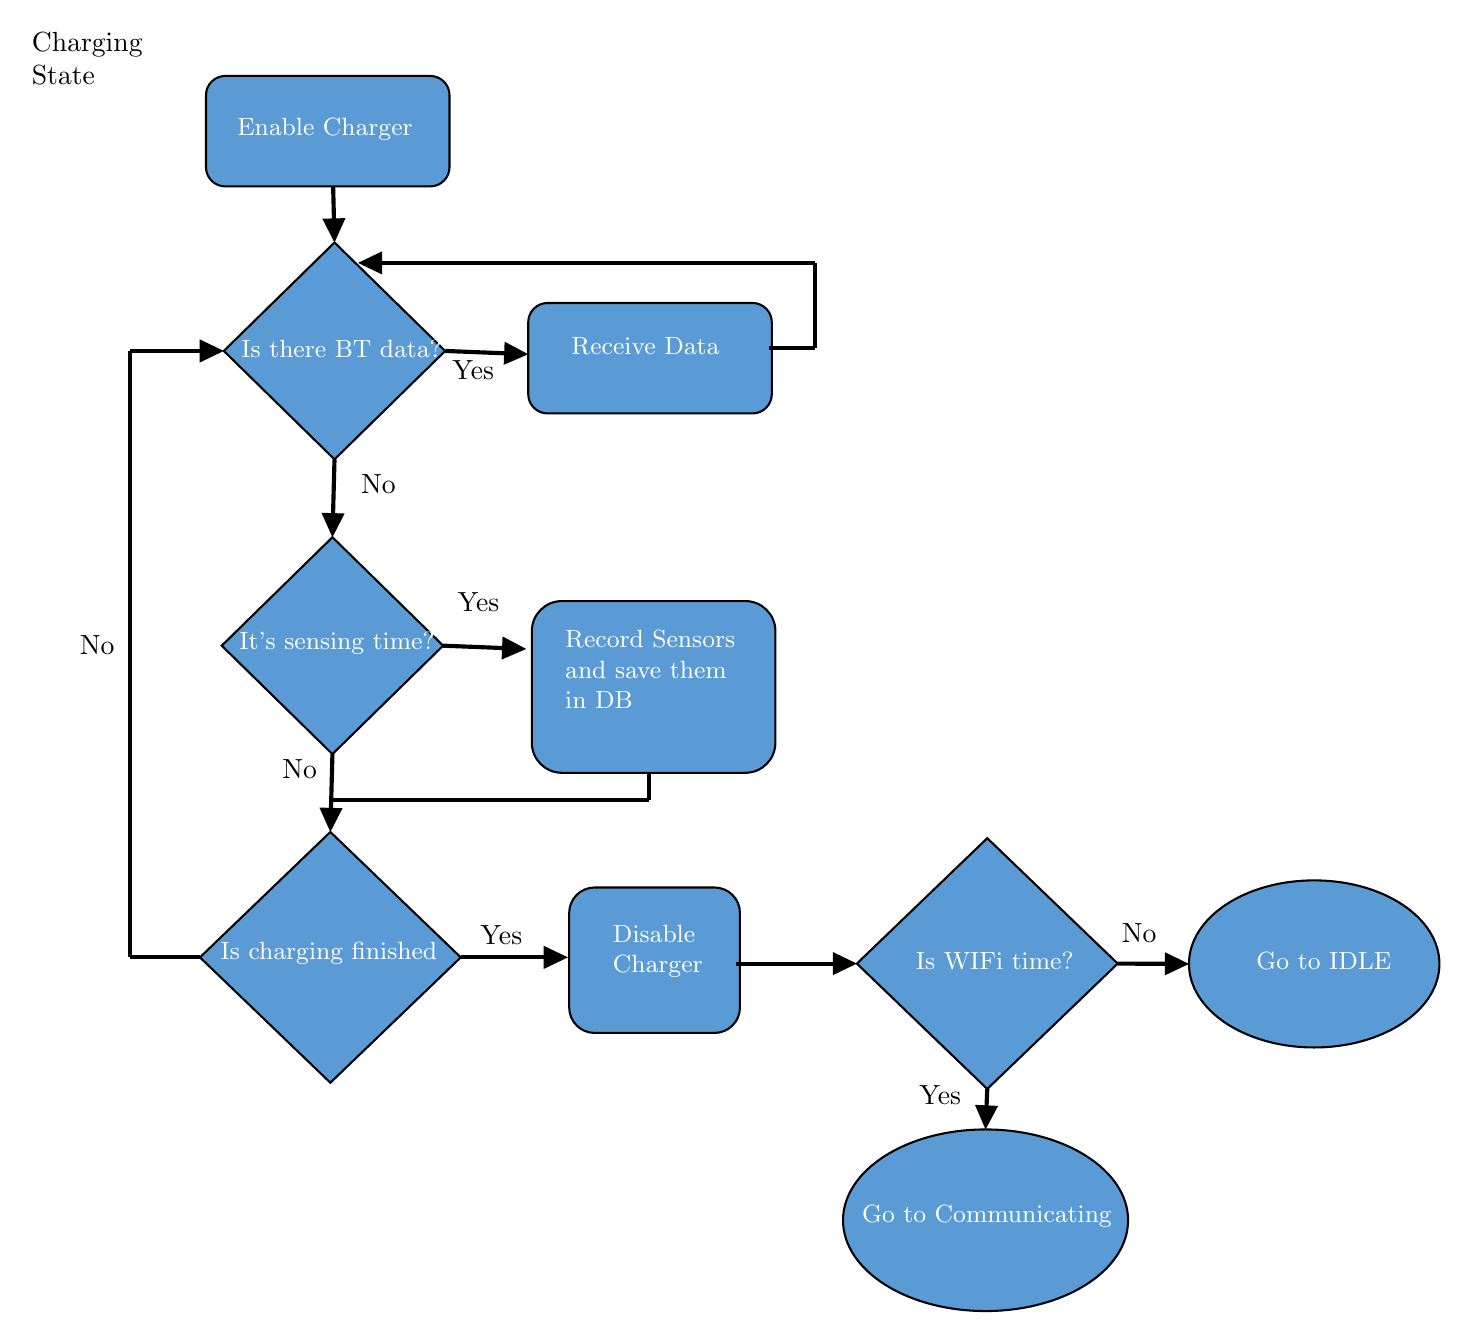
\begin{tikzpicture}[x=0.75pt,y=0.75pt,yscale=-1,xscale=1]
%uncomment if require: \path (0,636); %set diagram left start at 0, and has height of 636

%Flowchart: Alternative Process [id:dp9678129498459402] 
\draw  [color={rgb, 255:red, 0; green, 0; blue, 0 }  ,draw opacity=1 ][fill={rgb, 255:red, 91; green, 155; blue, 213 }  ,fill opacity=1 ] (91.4,40.07) .. controls (91.4,34.93) and (95.57,30.76) .. (100.71,30.76) -- (199.44,30.76) .. controls (204.58,30.76) and (208.75,34.93) .. (208.75,40.07) -- (208.75,74.66) .. controls (208.75,79.81) and (204.58,83.98) .. (199.44,83.98) -- (100.71,83.98) .. controls (95.57,83.98) and (91.4,79.81) .. (91.4,74.66) -- cycle ;
%Flowchart: Decision [id:dp08776045784490272] 
\draw  [fill={rgb, 255:red, 91; green, 155; blue, 213 }  ,fill opacity=1 ] (153.33,111) -- (206.67,163.25) -- (153.33,215.5) -- (100,163.25) -- cycle ;
%Flowchart: Alternative Process [id:dp10215954497716018] 
\draw  [color={rgb, 255:red, 0; green, 0; blue, 0 }  ,draw opacity=1 ][fill={rgb, 255:red, 91; green, 155; blue, 213 }  ,fill opacity=1 ] (246.67,149.45) .. controls (246.67,144.31) and (250.84,140.14) .. (255.98,140.14) -- (354.71,140.14) .. controls (359.85,140.14) and (364.02,144.31) .. (364.02,149.45) -- (364.02,184.04) .. controls (364.02,189.18) and (359.85,193.35) .. (354.71,193.35) -- (255.98,193.35) .. controls (250.84,193.35) and (246.67,189.18) .. (246.67,184.04) -- cycle ;
%Flowchart: Decision [id:dp47313701299195743] 
\draw  [fill={rgb, 255:red, 91; green, 155; blue, 213 }  ,fill opacity=1 ] (152.33,253) -- (205.67,305.25) -- (152.33,357.5) -- (99,305.25) -- cycle ;
%Flowchart: Alternative Process [id:dp5230664698955705] 
\draw  [color={rgb, 255:red, 0; green, 0; blue, 0 }  ,draw opacity=1 ][fill={rgb, 255:red, 91; green, 155; blue, 213 }  ,fill opacity=1 ] (248.4,298.24) .. controls (248.4,290.24) and (254.88,283.76) .. (262.88,283.76) -- (351.27,283.76) .. controls (359.27,283.76) and (365.75,290.24) .. (365.75,298.24) -- (365.75,352.02) .. controls (365.75,360.02) and (359.27,366.5) .. (351.27,366.5) -- (262.88,366.5) .. controls (254.88,366.5) and (248.4,360.02) .. (248.4,352.02) -- cycle ;
%Flowchart: Decision [id:dp6604820106345477] 
\draw  [fill={rgb, 255:red, 91; green, 155; blue, 213 }  ,fill opacity=1 ] (151.33,395) -- (214.17,455.42) -- (151.33,515.83) -- (88.5,455.42) -- cycle ;
%Flowchart: Alternative Process [id:dp41355941257164264] 
\draw  [color={rgb, 255:red, 0; green, 0; blue, 0 }  ,draw opacity=1 ][fill={rgb, 255:red, 91; green, 155; blue, 213 }  ,fill opacity=1 ] (266.4,434.02) .. controls (266.4,427.25) and (271.89,421.76) .. (278.66,421.76) -- (336.4,421.76) .. controls (343.18,421.76) and (348.67,427.25) .. (348.67,434.02) -- (348.67,479.57) .. controls (348.67,486.34) and (343.18,491.83) .. (336.4,491.83) -- (278.66,491.83) .. controls (271.89,491.83) and (266.4,486.34) .. (266.4,479.57) -- cycle ;
%Flowchart: Decision [id:dp4443865172272685] 
\draw  [fill={rgb, 255:red, 91; green, 155; blue, 213 }  ,fill opacity=1 ] (467.83,398) -- (530.67,458.42) -- (467.83,518.83) -- (405,458.42) -- cycle ;
%Shape: Ellipse [id:dp14488660606305936] 
\draw  [fill={rgb, 255:red, 91; green, 155; blue, 213 }  ,fill opacity=1 ] (565,458.58) .. controls (565,436.35) and (592.01,418.33) .. (625.33,418.33) .. controls (658.65,418.33) and (685.67,436.35) .. (685.67,458.58) .. controls (685.67,480.81) and (658.65,498.83) .. (625.33,498.83) .. controls (592.01,498.83) and (565,480.81) .. (565,458.58) -- cycle ;
%Shape: Ellipse [id:dp47020080832752176] 
\draw  [fill={rgb, 255:red, 91; green, 155; blue, 213 }  ,fill opacity=1 ] (398.33,582.08) .. controls (398.33,557.92) and (429.08,538.33) .. (467,538.33) .. controls (504.92,538.33) and (535.67,557.92) .. (535.67,582.08) .. controls (535.67,606.25) and (504.92,625.83) .. (467,625.83) .. controls (429.08,625.83) and (398.33,606.25) .. (398.33,582.08) -- cycle ;
%Straight Lines [id:da8099961021885935] 
\draw [line width=1.5]    (152.67,83.83) -- (153.24,107) ;
\draw [shift={(153.33,111)}, rotate = 268.59000000000003] [fill={rgb, 255:red, 0; green, 0; blue, 0 }  ][line width=0.08]  [draw opacity=0] (11.61,-5.58) -- (0,0) -- (11.61,5.58) -- cycle    ;
%Straight Lines [id:da8112299877056122] 
\draw [line width=1.5]    (153.33,215.5) -- (152.44,249) ;
\draw [shift={(152.33,253)}, rotate = 271.53] [fill={rgb, 255:red, 0; green, 0; blue, 0 }  ][line width=0.08]  [draw opacity=0] (11.61,-5.58) -- (0,0) -- (11.61,5.58) -- cycle    ;
%Straight Lines [id:da9373430912302989] 
\draw [line width=1.5]    (152.33,357.5) -- (151.44,391) ;
\draw [shift={(151.33,395)}, rotate = 271.53] [fill={rgb, 255:red, 0; green, 0; blue, 0 }  ][line width=0.08]  [draw opacity=0] (11.61,-5.58) -- (0,0) -- (11.61,5.58) -- cycle    ;
%Straight Lines [id:da2149756219882788] 
\draw [line width=1.5]    (214.17,455.42) -- (261.75,455.42) ;
\draw [shift={(265.75,455.42)}, rotate = 180] [fill={rgb, 255:red, 0; green, 0; blue, 0 }  ][line width=0.08]  [draw opacity=0] (11.61,-5.58) -- (0,0) -- (11.61,5.58) -- cycle    ;
%Straight Lines [id:da34053630869138507] 
\draw [line width=1.5]    (346.67,458.42) -- (401,458.42) ;
\draw [shift={(405,458.42)}, rotate = 180] [fill={rgb, 255:red, 0; green, 0; blue, 0 }  ][line width=0.08]  [draw opacity=0] (11.61,-5.58) -- (0,0) -- (11.61,5.58) -- cycle    ;
%Straight Lines [id:da16684532731244062] 
\draw [line width=1.5]    (530.67,458.42) -- (561,458.56) ;
\draw [shift={(565,458.58)}, rotate = 180.28] [fill={rgb, 255:red, 0; green, 0; blue, 0 }  ][line width=0.08]  [draw opacity=0] (11.61,-5.58) -- (0,0) -- (11.61,5.58) -- cycle    ;
%Straight Lines [id:da7917152286796634] 
\draw [line width=1.5]    (467.83,518.83) -- (467.17,534.34) ;
\draw [shift={(467,538.33)}, rotate = 272.45] [fill={rgb, 255:red, 0; green, 0; blue, 0 }  ][line width=0.08]  [draw opacity=0] (11.61,-5.58) -- (0,0) -- (11.61,5.58) -- cycle    ;
%Straight Lines [id:da0975530461334484] 
\draw [line width=1.5]    (206.67,163.25) -- (242.67,164.68) ;
\draw [shift={(246.67,164.83)}, rotate = 182.27] [fill={rgb, 255:red, 0; green, 0; blue, 0 }  ][line width=0.08]  [draw opacity=0] (11.61,-5.58) -- (0,0) -- (11.61,5.58) -- cycle    ;
%Straight Lines [id:da2866710881613719] 
\draw [line width=1.5]    (384.67,120.83) -- (168.67,120.83) ;
\draw [shift={(164.67,120.83)}, rotate = 360] [fill={rgb, 255:red, 0; green, 0; blue, 0 }  ][line width=0.08]  [draw opacity=0] (11.61,-5.58) -- (0,0) -- (11.61,5.58) -- cycle    ;
%Straight Lines [id:da8834119174259045] 
\draw [line width=1.5]    (384.67,161.83) -- (362.67,161.83) ;
%Straight Lines [id:da2369723315178247] 
\draw [line width=1.5]    (384.67,120.83) -- (384.67,161.83) ;
%Straight Lines [id:da32389857128517274] 
\draw [line width=1.5]    (205.67,305.25) -- (241.67,306.68) ;
\draw [shift={(245.67,306.83)}, rotate = 182.27] [fill={rgb, 255:red, 0; green, 0; blue, 0 }  ][line width=0.08]  [draw opacity=0] (11.61,-5.58) -- (0,0) -- (11.61,5.58) -- cycle    ;
%Straight Lines [id:da5124134741686268] 
\draw [line width=1.5]    (151.75,379.75) -- (304.75,379.75) ;
%Straight Lines [id:da23027306149649363] 
\draw [line width=1.5]    (304.75,379.75) -- (304.75,366.75) ;
%Straight Lines [id:da41405767669110993] 
\draw [line width=1.5]    (54.75,163.25) -- (96,163.25) ;
\draw [shift={(100,163.25)}, rotate = 180] [fill={rgb, 255:red, 0; green, 0; blue, 0 }  ][line width=0.08]  [draw opacity=0] (11.61,-5.58) -- (0,0) -- (11.61,5.58) -- cycle    ;
%Straight Lines [id:da8598782000538134] 
\draw [line width=1.5]    (54.75,163.25) -- (54.75,455.42) ;
%Straight Lines [id:da1594081040335633] 
\draw [line width=1.5]    (88.5,455.42) -- (54.75,455.42) ;

% Text Node
\draw (104.99,49.44) node [anchor=north west][inner sep=0.75pt]  [font=\small,color={rgb, 255:red, 255; green, 255; blue, 255 }  ,opacity=1 ] [align=left] {{\small Enable Charger}};
% Text Node
\draw (6,8) node [anchor=north west][inner sep=0.75pt]   [align=left] {Charging\\State};
% Text Node
\draw (106.99,156.44) node [anchor=north west][inner sep=0.75pt]  [font=\small,color={rgb, 255:red, 255; green, 255; blue, 255 }  ,opacity=1 ] [align=left] {{\small Is there BT data?}};
% Text Node
\draw (265.99,155.44) node [anchor=north west][inner sep=0.75pt]  [font=\small,color={rgb, 255:red, 255; green, 255; blue, 255 }  ,opacity=1 ] [align=left] {{\small Receive Data}};
% Text Node
\draw (105.99,297.44) node [anchor=north west][inner sep=0.75pt]  [font=\small,color={rgb, 255:red, 255; green, 255; blue, 255 }  ,opacity=1 ] [align=left] {{\small It's sensing time?}};
% Text Node
\draw (262.99,296.44) node [anchor=north west][inner sep=0.75pt]  [font=\small,color={rgb, 255:red, 255; green, 255; blue, 255 }  ,opacity=1 ] [align=left] {{\small Record Sensors}\\and save them\\in DB};
% Text Node
\draw (96.99,446.44) node [anchor=north west][inner sep=0.75pt]  [font=\small,color={rgb, 255:red, 255; green, 255; blue, 255 }  ,opacity=1 ] [align=left] {{\small Is charging finished}};
% Text Node
\draw (285.99,438.44) node [anchor=north west][inner sep=0.75pt]  [font=\small,color={rgb, 255:red, 255; green, 255; blue, 255 }  ,opacity=1 ] [align=left] {{\small Disable}\\Charger};
% Text Node
\draw (431.99,451.44) node [anchor=north west][inner sep=0.75pt]  [font=\small,color={rgb, 255:red, 255; green, 255; blue, 255 }  ,opacity=1 ] [align=left] {{\small Is WIFi time?}};
% Text Node
\draw (595.99,451.44) node [anchor=north west][inner sep=0.75pt]  [font=\small,color={rgb, 255:red, 255; green, 255; blue, 255 }  ,opacity=1 ] [align=left] {{\small Go to IDLE}};
% Text Node
\draw (405.99,573.44) node [anchor=north west][inner sep=0.75pt]  [font=\small,color={rgb, 255:red, 255; green, 255; blue, 255 }  ,opacity=1 ] [align=left] {{\small Go to Communicating}};
% Text Node
\draw (208.67,166.25) node [anchor=north west][inner sep=0.75pt]   [align=left] {Yes};
% Text Node
\draw (164.67,221.25) node [anchor=north west][inner sep=0.75pt]   [align=left] {No};
% Text Node
\draw (211.17,278.25) node [anchor=north west][inner sep=0.75pt]   [align=left] {Yes};
% Text Node
\draw (126.67,358.75) node [anchor=north west][inner sep=0.75pt]   [align=left] {No};
% Text Node
\draw (222.17,438.75) node [anchor=north west][inner sep=0.75pt]   [align=left] {Yes};
% Text Node
\draw (433.67,515.75) node [anchor=north west][inner sep=0.75pt]   [align=left] {Yes};
% Text Node
\draw (531.17,437.75) node [anchor=north west][inner sep=0.75pt]   [align=left] {No};
% Text Node
\draw (29.17,298.75) node [anchor=north west][inner sep=0.75pt]   [align=left] {No};


\end{tikzpicture}